\documentclass[
  journal=small,
  manuscript=article-type,  % Use a - if you need a space e.g. "research-article"
  year=2020,
  volume=37,
]{cup-journal}

\usepackage{amsmath}
\usepackage[nopatch]{microtype}
\usepackage{booktabs}
%\usepackage{hyperref}

\title{Deepfakes: What Are The Impacts?}

\author{In Woo Park}
\affiliation{ICS 691D, UH MANOA, Honolulu, HI}
\email[F. Author]{inwoo@hawaii.edu}

%\addbibresource{example.bib}

\keywords{deep fakes, detection, social} 

\begin{document}

\begin{abstract}
Deepfake technology has contributed in the creation of fake content. In an age where an emphasis is placed on fake news and disinformation, it is important now than ever in viewing visual and auditory media with a critical lens. We take on this challenge by observing the influence of deepfake disinformation through surface layer coverage of deepfake generation, deep fake detection with human participants, and deepfake societal impacts in the political climate. 
\end{abstract}

\section{Introduction}
On April 18, 2019, a video of former President Barack Obama went viral world-wide (Vaccari 2020). The reason for the video's popularity is attributed to Barack Obama's unorthodox statements such as "Killmonger was right", "Ben Carson is in the sunken place" and "President Trump is a total and complete dipshit." To many people, this video was their introduction to the world of deepfakes and its possibilities. Although deepfakes have been around prior to this video, the video played a significant role in providing visibility to this alarming phenomenon. 

The word deepfake is a portmanteau\footnote{a word blending the sounds and combining the meanings of two others} of the words, "deep learning"\footnote{a subset of Machine Learning which uses neural networks to train a model} and "fakes". Therefore, when we describe a piece of content as a deepfake, we declare that the content (i.e., visual, audio) itself has been created, fabricated, or edited with the intent to deceive the viewer is some-way (Kietzmann 2020). The impact of deepfakes and its potential to cause social and political discourse is ever more important today. In the age where the court of public opinion is highly dependant on social media, it is more important than ever to discuss the credibility of media and to view every content with a critical lens. This paper will review the influence of deepfake disinformation by observing deepfake generation, detection, and its social impact. 

\section{Deepfake Generation}
There is extensive literature that explains each type of deepfake that can be generated and what type of Machine Learning method can be employed for that particular deepfake (Table 1). If we review the types of deepfakes presented by Kietzmann and Masood, we can categorize PBODV as a lip sync-based deepfake. 

There are multiple types of machine learning techniques that can be used to generate lip sync-based deepfakes. Each technique depends on a technical balance between output quality of the deepfake and the limitations it opposes. Masood's (2022) paper provides an overview of the techniques used in generating lip sync-based deepfakes. These techniques are RNN, Encoder-decoder CNN, Temporal GAN, and 3DMM. However, out of all the techniques presented, recurrent neural networks (single-layer unidirectional LSTM) produces the highest resolution in output quality at 2048x1024 (Masood 2022). The RNN model learns to map between mouth shape and audio features per frame and uses frame re-selection to fill textures around the mouth. This approach also requires post-processing edits such as smoothing jaw location or re-timing the video to match audio/vocal pauses to polish the deepfake (Suwajanakorn et al. in Masood 2022). It is important to mention that the limitations of RNN include: 1) requiring large data set for training, 2) sensitivity to 3D movement of the head, and 3) no control over facial expressions. Luckily, there is a  sufficient amount of available online footage of Barack Obama for training data. In the case of PBODV, it is likely that the footage of Obama is from a real video but his mouth is faked to lip-sync with the audio sound bite of Jordan Peele stating pop-culture references.

\section{Deepfake Detection: Humans}
Deepfakes have the ability to spread misinformation. Therefore, we must do our due diligence in checking the credibility of video and audio media before considering an instance as fact. However, how well does a person perform in detecting deepfake content? We observe three studies that attempt to answer this question.

\subsection{Deceived, Not Deceived, or Uncertain}
The first study tackles the issue head-on with a similar hypothesis as to what we stated previously (Vaccari 2020). The study had a representative sample (N=2,005) where after being presented with some type of video, a participant is asked to measure the truthfulness of the deepfake by responding to a questionnaire. Participants were (evenly) split into three groups. The first group was presented with a 4-second version of PBODV (Obama calls Trump a dipshit). The second group was presented with a 26-second version of PBODV (the entire deepfake without the educational reveal). The third group was the full video with the educational reveal. The study admits that a big limitation was that there was no control group. The participants were then asked to rate their reaction to the video as, not deceived, uncertain, or deceived. 

The overall results of each group revealed that 50.8\% of people were not deceived by the deepfake, 33.2\% of people were uncertain, and 16\% of people were deceived. Following the same order, the 4-second group had a 50.1/35.1/14.9 split, the 26-second group had a 46.7/36.9/16.4 split, and the full video had a 55.6/27.5/16.9 split. The study concludes that although political deepfakes may not necessarily deceive individuals, it may sow uncertainty which may reduce trust in news on social media. 

\subsection{Fabricated or Original}
The next study researches deeper into the ability of humans to detect political deepfakes from transcripts, audio, and video (Groh 2022). Compared to the previous study, this study had a larger sample size (N = 41,822) and three different deepfake content categories (224 authentic and fabricated). Participants were asked to label a video as fabricated or non-fabricated based on their reaction to political speeches. The speeches were randomized to be either type of media category (transcript, audio, video). 

It was reported that the realism heuristic, which suggests that people tend to trust video over text, was present in their results as people were, "significantly more accurate at identifying authentic speeches as authentic when the speeches include audio and visual modalities as opposed to only text." Participants on distinguishing authentic from fabricated content, had an accuracy of 57\% for political speech transcripts, 66\% for videos with subtitles, and 82\% for videos with audio.

\subsection{By Partisan}
The final study conducted two experiments with a sample size of N = 5,750 (Barari 2021). The first experiement had participants with a news feed of video clips, audio clips, and text headlines of candidates in the 2020 Democratic presidential primary. A deepfake of one of the candidate may or may not been inserted in the news feed. The second experiment had the same participants scroll through a news feed of eight videos which were randomized to either contain no deepfakes, two deepfakes, or six deepfakes. Participants were then asked to detect which clips were authentic and which were fabricated. The deepfakes used were either face swaps or lip syncs. 

Participants who were in the no deepfake category had an accuracy of 58\% with a 22.27\% false positive rate, participants in the two deepfake category had an accuracy of 57.02\% with 22.05\% false positive rate, and participants in the six deepfake category had an accuracy of 54.47\% with a 19.23\% false positive rate. The study goes further to explain other interesting findings such as when the study grouped the the accuracy of participants by political party, Republicans appeared to marginally outperform Democrats and Independents (roughly 5-6\%). However, this gap is exacerbated when this phenomenon is observed in only real videos. For instance, a real video of Barack Obama insinuating a political motive was believed to be real by 58\% of Republicans, compared to 22\% of Democrats. Two other real video instances had similar results (Joe Biden stuttering 78R/56D, and Donald Trump's COVID-19 annoucement 81R/58D). 

\subsection{Performance}

Previously we asked ourselves, how well does a person perform in detecting deepfake content? Between the three studies presented, we can conclude that the ability for a person to detect deepfake content depends on the circumstance. 

The first study used PBODV as the only deepfake example and asked participants to rate their authenticity reaction. Should it be alarming that roughly 50\% of participants considered themselves not deceived by the deepfake? Not necessarily if we consider that 30\% of participants considered themselves as uncertain. It is better for a participant to be in the state of uncertainty than deceived as it means there isn't enough information for them to decide (indicating critical thought). 

The second study tells us that the ability for a person to detect deepfake content depends on the type of content. Participants in this study showed that on average, it was easier for them to detect deepfakes for political speeches with video and audio than any other medium (transcripts, subtitles).

Lastly, the third study tells us in a simulated instance (scrolling through a newsfeed), even when no deepfake is present, participants are only 8\% better than random chance at detection, with an average gap of 5\% between Republicans and Democrats. 

All in all, the studies presented seem to indicate that fabricated videos of public officials are credible up-to 50\% of the American public (Barari 2021). Without applying a harsh generalization, humans are average in detecting deepfake content.  

\section{Social Impact}
Vacarri (2020) tells us that although people were unlikely to be completely misled by deepfakes, exposure to deepfakes increased uncertainty in general. In other words, deepfakes made participants less trustworthy of media. This conclusion is consistent with the research by Ahmed (2021) as well who conducted a similar study to Vacarri (2020). The findings of their research suggest that exposure to deepfakes are positively related to social media news skepticism. However, those who frequented social media as news platform were more trustful of the medium in contrast. What could explain this phenomenon? Perhaps it could be due to confirmation bias. 

Hameleer (2022) conducted a similar study in which participants (N = 1,244) were provided randomized political speeches to view and then asked to answer a set of questions. Each political speech had some form of disinformation embedded into the video or audio. The participants were then asked questions about the credibility and authenticity of the disinformation, their agreement with the political statement, and their evaluation of the politician. The results of the study found that disinformation was more effective in affecting credibility ratings and evaluations if the participant agreed with the political statement. This is likely due to disinformation reinforcing existing beliefs if it aligned with person's prior beliefs. In \textbf{Figure 1}, we can see that Hameleer's (2022) study showed an almost 1:1 linear mapping between prior issue agreement and agreement with the disinformation's statement. In \textbf{Figure 2}, we can also see that the higher a participant agreed with an issue, the more likely they were to consider it credible. These instances were interpreted as confirmation bias' for deepfakes. 

Deepfakes also have interpersonal consequences (Hancock 2021). It's entirely plausible for a deepfake to potentially change a person's memory or modify a person's attitude toward a political figure. Dobber's (2021) study (N = 278) attempted to find the impact of deepfakes on political attitudes. In a similar design, participants were split into two groups that either saw a deepfake video or a control video and then asked questions afterwards. The study found that the experimental group had significantly worse attitudes towards the politician after watching the deepfake footage, but negligible attitude change towards the politicians political party. 

\section{Conclusion}
Deepfake technology is state-of-the-art. Using deep learning models, anyone and everyone can create deepfake media. In our paper, we discussed the influence of deepfake disinformation by observing deepfake generation, detection, and its social impact. A common trend among the studies reviewed showed that deepfakes were usually associated with politics and disinformation. These discussions are necessary in our current political climate where we have placed a strong emphasis on detecting fake news mediums and being critical of news on social media. Although the participants across the studies reported and increase in skepticism and distrust of media after viewing deepfakes, these aren't the people the deepfakes are targeting. As we seen from Hameleer (2022) and Hancock (2021), political attitude is more likely to be swayed by confirmation bias and prior issue agreement with a dis-informed statement. Therefore, we must apply a critical lens on every form of news medium. Not all deepfakes are malicious, but all deepfakes are deceitful. 

A limitation of our paper is our approach towards deepfake technology. If this paper were to be visited in the future, we would add more emphasis on other deep learning methods for generating deepfakes.  

\begin{table}[hbt!]
\begin{threeparttable}
\caption{Categorization of Articles}
\label{deepfake_type}
\begin{tabular}{llll}
\toprule
\headrow Reference & Category & Data Collection Type & Data Collection Design  \\
\midrule
Ahmed 2021 & Social Impact & Survey & Strong\\ 
\midrule
Barari 2021 & Human Detection & Survey & Strong\\ 
\midrule
Dobber 2021 & Social Impact & Survey & Moderate\\ 
\midrule
Groh 2022 & Human Detection & Survey & Strong\\ 
\midrule
Hameleers 2022 & Social Impact & Survey & Strong\\ 
\midrule
Hancock 2021 & Social Impact & Survey & Moderate\\ 
\midrule
Kietzmann 2020 & Generation Explained & Technical & Moderate\\ 
\midrule
Masood 2022 & Generation and Detection & Technical & Strong\\ 
\midrule
Vaccari 2020 & Human Detection & Survey & Moderate\\ 
\bottomrule
\end{tabular}
\end{threeparttable}
\end{table}

These studies were included based on its relation to deepfake detection or deepfake social impact. Other studies were considered but not used if their data collection design was $<$ N = 200 participants for the survey papers. The two technical papers were included because they thoroughly explained deepfake detection techniques. 

%See example table in Table~\ref{table_example}.
\begin{table}[hbt!]
\begin{threeparttable}
\caption{Types of Deepfakes}
\label{deepfake_type}
\begin{tabular}{llll}
\toprule
\headrow Type & Description \\
\midrule
Photo & Face and body-swapping\\ 
\midrule
Audio & Voice-swapping\\ 
\midrule
Audio & Text-to-Speech\\ 
\midrule
Video & Face-swapping\\ 
\midrule
Video & Face-morphing\\ 
\midrule
Video & Full-body puppetry\\ 
\midrule
Audio and Video & Lip-syncing\\ 
\bottomrule
\end{tabular}
\end{threeparttable}
\end{table}

\begin{figure*}
\centering
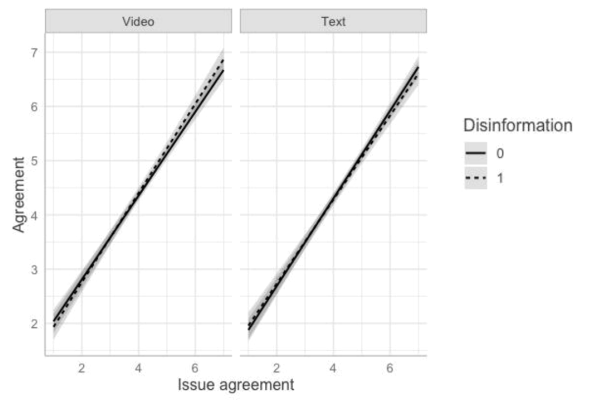
\includegraphics[width=0.6\linewidth]{leaf.png}
\caption{The effects of textual deepfakes on prior issue agreement by levels of agreement with disinformation's statement (Hameleer 2022).}
\label{fig_wide}
\end{figure*}

\begin{figure*}
\centering
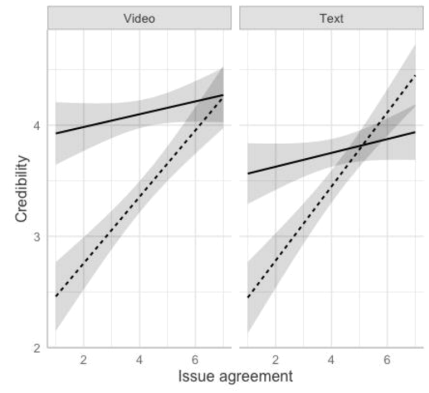
\includegraphics[width=0.45\linewidth]{leaf2.png}
\caption{The effects of textual deepfakes on credibility by levels of agreement with disinformation's statement (Hameleer 2022).}
\label{fig_wide}
\end{figure*}

\newpage
\begin{thebibliography}{9}

\bibitem{Journal}
Ahmed, S. (2021). Navigating the maze: Deepfakes, cognitive ability, and social media news skepticism. new media \& society, 14614448211019198.

\bibitem{Journal}
Barari, S., Lucas, C., \& Munger, K. (2021). Political deepfakes are as credible as other fake media and (sometimes) real media.

\bibitem{Journal}
Dobber, T., Metoui, N., Trilling, D., Helberger, N., \& de Vreese, C. (2021). Do (microtargeted) deepfakes have real effects on political attitudes?. The International Journal of Press/Politics, 26(1), 69-91.

\bibitem{Journal}
Groh, M., Sankaranarayanan, A., \& Picard, R. (2022). Human detection of political deepfakes across transcripts, audio, and video. arXiv preprint arXiv:2202.12883.

\bibitem{Journal}
Hameleers, M., van der Meer, T. G., \& Dobber, T. (2022). You Won’t Believe What They Just Said! The Effects of Political Deepfakes Embedded as Vox Populi on Social Media. Social Media+ Society, 8(3), 20563051221116346.

\bibitem{Journal}
Hancock, J. T., \& Bailenson, J. N. (2021). The social impact of deepfakes. Cyberpsychology, behavior, and social networking, 24(3), 149-152.

\bibitem{Journal}
Kietzmann, J., Lee, L. W., McCarthy, I. P., \& Kietzmann, T. C. (2020). Deepfakes: Trick or treat?. Business Horizons, 63(2), 135-146.

\bibitem{Journal}
Masood, M., Nawaz, M., Malik, K. M., Javed, A., Irtaza, A., \& Malik, H. (2022). Deepfakes Generation and Detection: State-of-the-art, open challenges, countermeasures, and way forward. Applied Intelligence, 1-53.

\bibitem{Journal}
Vaccari, C., \& Chadwick, A. (2020). Deepfakes and disinformation: Exploring the impact of synthetic political video on deception, uncertainty, and trust in news. Social Media Society, 6(1), 2056305120903408.

\end{thebibliography}

\end{document}
